\documentclass{beamer}
\usetheme{metropolis}
\setbeamercovered{transparent}

\usepackage{amsmath, amssymb, amsthm}
\usepackage{graphicx}
\usepackage[scr]{rsfso}
\usepackage{forloop}

\def\C{\mathbb{C}}
\def\R{\mathbb{R}}
\def\Q{\mathbb{Q}}
\def\Z{\mathbb{Z}}
\def\N{\mathbb{N}}

\title{
    The Trapezoidal Method
}
\subtitle{
    Numerically solving first order ordinary differential equations
}
\author{Satvik Saha}
\institute{
    Final project for MA3105: Numerical Analysis \\
    Indian Institute of Science Education and Research, Kolkata
}
\date{November 23, 2021}

\begin{document}
    \maketitle

    \section{The initial value problem}

    \begin{frame}{The initial value problem}
    Given the derivative of a function $y$ and an initial value $y(x_0)$, we wish to
    reconstruct the curve $y(x)$. \[
        y'(x) = f(x, y(x)), \qquad y(x_0) = y_0.
    \] \\~\\

    For example, \[
        y'(x) = y - x, \qquad y(0) = \frac{2}{3}.
    \]
    \end{frame}

    \begin{frame}{The analytic solution}
        If \[
            y'(x) = p(x)y(x) + q(x), \qquad y(x_0) = y_0,
        \] then \[
            y(x) = y_0 + g(x)\int_{x_0}^x \frac{q(x)}{g(x)} \:dx, \qquad g(x) = \exp
            \int_{a}^x p(x)\:dx.
        \] \\~\\

        In our example, \[
            y(x) = \frac{2}{3} + e^x\int_0^x xe^{-x}\:dx = 1 + x - \frac{1}{3}e^x.
        \] 
    \end{frame}

    \begin{frame}{The big picture}
        Examine the differential equation \[
            y'(x) = f(x, y(x)).
        \] This can be read as follows. \\~\\

        \begin{quote}
            Given a point $(x, y)$ on a solution curve $y(x)$, the tangent drawn to
            the curve at that point has slope $f(x, y)$.
        \end{quote}

        Thus, we can assign a vector with slope $f(x, y)$ to each point $(x, y)$ on
        the plane; this gives us a \emph{direction field}. Any solution $y(x)$ will
        fit neatly into this field.
    \end{frame}

    \begin{frame}[plain]
        \begin{center}
            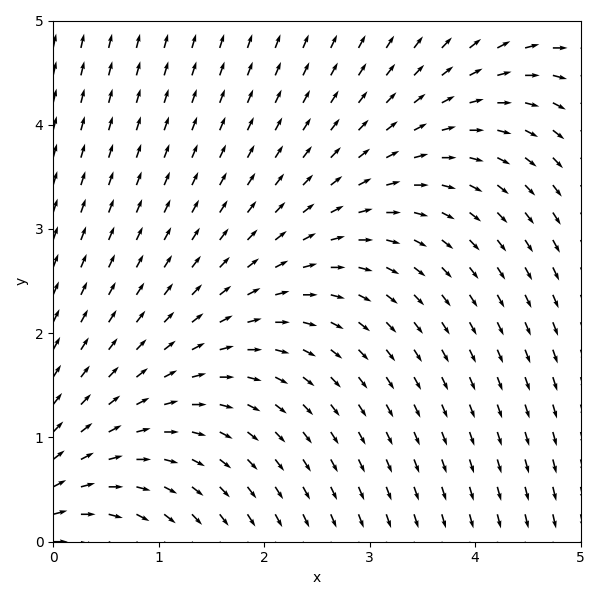
\includegraphics[width=0.85\textwidth]{./img/directionfield.png}
        \end{center}
    \end{frame}
    
    \begin{frame}{Joining the dots}
        \begin{enumerate}
            \item Start at $(x_0, y_0)$, and move along the tangent vector there by a
            small step to reach $(x_1, y_1)$.
            \item Join these points, and repeat.
        \end{enumerate}

        The resulting curve closely approximates a solution to the initial value
        problem.

        This `works' because for a smooth curve $y(x)$, the tangent line closely
        approximates the curve.
    \end{frame}

    \begin{frame}[plain]
        \begin{center}
            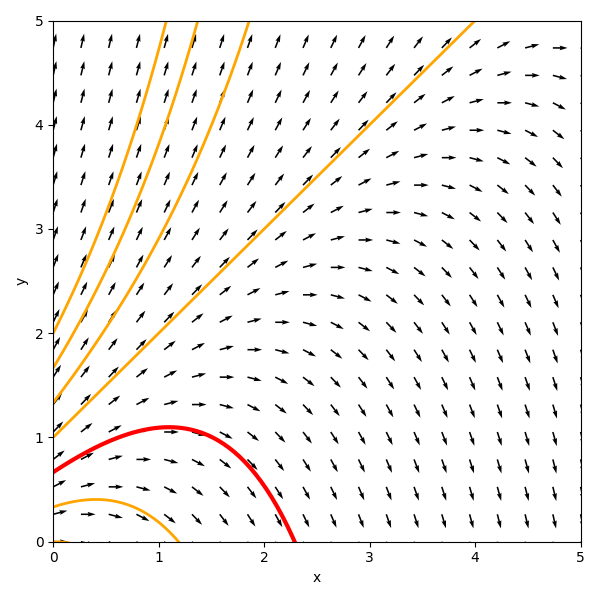
\includegraphics[width=0.85\textwidth]{./img/directionfield_curves.png}
        \end{center}
    \end{frame}
    

    \section{Iterative methods}

    \begin{frame}{Euler's method}
        Recall that \[
            y'(x) = \lim_{h \to 0} \frac{y(x + h) - y(x)}{h}.
        \] \\~\\

        Thus, we can make the \emph{forward} and \emph{backward} approximations,
        \[
            y'(x) \approx \frac{y(x + h) - y(x)}{h} \approx \frac{y(x) - y(x -
            h)}{h}.
        \] 
    \end{frame}

    \begin{frame}{Euler's method}
        This gives two ways of stepping along the $x$-axis, an explicit one and an
        implicit one. \begin{align*}
            y(x + h) &\approx y(x) + h\cdot y'(x), \\
            y(x + h) &\approx y(x) + h\cdot y'(x + h).
        \end{align*}

        More precisely, Taylor's theorem gives us \[
            y(x + h) = y(x) + h\cdot y'(x) + \mathcal{O}(h^2).
        \] 
    \end{frame}

    \begin{frame}{Euler's method}
        Suppose that we wish to approximate the values of $y(x_i)$ for $x_i = x_0 +
        ih$, $0 \leq i \leq N$. Euler's method gives the scheme \[
            y_{i + 1} = y_i + h\cdot f(x_i, y_i).
        \] We claim that the values $y_i \approx y(x_i)$.
    \end{frame}
    
    \begin{frame}[plain]
        \begin{center}
            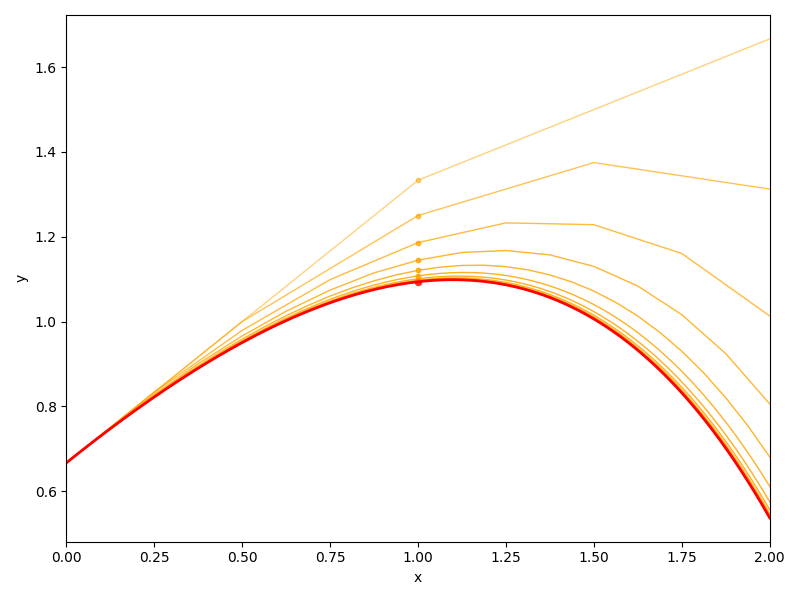
\includegraphics[width=\textwidth]{./img/euler.png}
        \end{center}
    \end{frame}
    
    
    \begin{frame}{Trapezoidal method}
        Recall our approximations \begin{align*}
            y(x + h) &\approx y(x) + h\cdot y'(x), \\
            y(x + h) &\approx y(x) + h\cdot y'(x + h).
        \end{align*}
        Taking their average, \[
            y(x + h) \approx y(x) + \frac{1}{2}h\cdot \Big[y'(x) + y'(x + h)\Big].
        \]
    \end{frame}

    \begin{frame}{Trapezoidal method}
        The following problems are essentially equivalent.
        \[
            y'(x) = f(x, y(x)), \qquad y(0) = y_0,
        \] 
        \[ \big\Updownarrow \] 
        \[
            y(x) = y_0 + \int_{x_0}^x f(x, y(x))\:dx.
        \] \\~\\

        The problem of integration can be split up into smaller pieces,
        \[
            y(x_{i + 1}) - y(x_i) = \int_{x_i}^{x_{i + 1}} f(x, y(x))\:dx.
        \] 
    \end{frame}

    \begin{frame}{Trapezoidal method}
        \begin{align*}
            y(x_{i + 1}) - y(x_i) &= \int_{x_i}^{x_{i + 1}} f(x, y(x))\:dx \\
            &\approx \frac{1}{2}h\cdot\Big[f(x_i, y(x_i)) + f(x_{i + 1},
            y(x_{i + 1}))\Big].
        \end{align*}
        
        This uses the trapezoidal method of approximating integrals,
        \[
            \int_a^b f(x)\:dx \approx \frac{b - a}{2}\cdot\Big[f(a) + f(b)\Big].
        \] 
    \end{frame}

    \begin{frame}{Trapezoidal method}
        The trapezoidal method gives the scheme \[
            y_{i + 1} = y_i + \frac{1}{2}h\cdot \Big[f(x_i, y_i) + f(x_{i + 1},
            y_{i + 1})\Big].
        \] \\~\\

        This does \emph{not} give $y_{i + 1}$ explicitly. Instead, we seek the root
        of \[
            g(t) = -t + y_i + \frac{1}{2}h\cdot \Big[f(x_i, y_i) + f(x_{i + 1},
            t)\Big].
        \] 
    \end{frame}

    \begin{frame}{Solving the implicit equation}
        One way of solving for $y_{i + 1}$ is using Newton's method. Set up a good
        initial guess using Euler's method, \[
            t_0 = y_i + h\cdot f(x_i, y_i),
        \] and proceed with \[
            t_{j + 1} = t_j - \frac{g(t_j)}{g'(t_j)}.
        \] We note that \[
            g'(t) = -1 + \frac{1}{2}h\cdot \frac{\partial f}{\partial y}(x_{i + 1},
            t).
        \] 
    \end{frame}
    
    \begin{frame}[plain]
        \begin{center}
            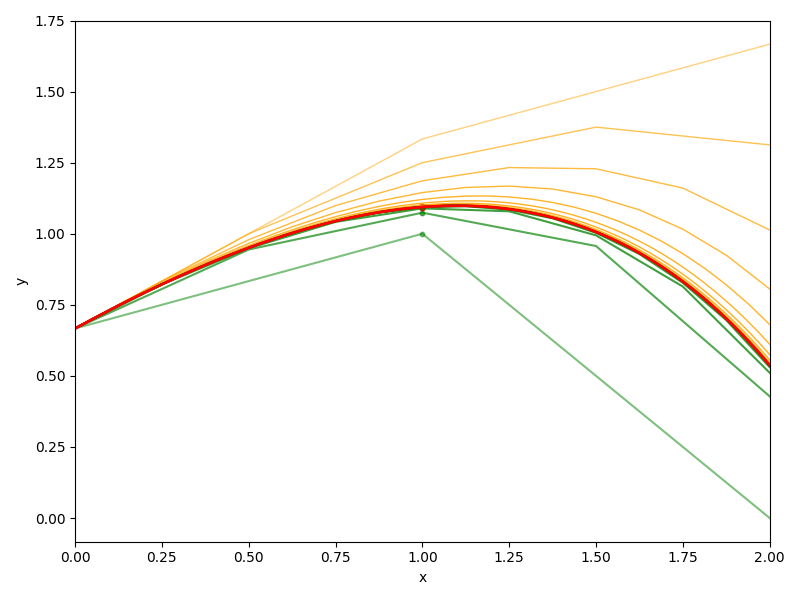
\includegraphics[width=\textwidth]{./img/trapezoidal.png}
        \end{center}
    \end{frame}


    \begin{frame}{An example by hand}
        Consider estimating $y(1)$ in one step (using $h = 1$) for the IVP \[
            y'(x) = y - x, \qquad y(0) = \frac{2}{3}.
        \] We solve the implicit equation for $y_1$. \[
            y_1 = \frac{2}{3} + \frac{1}{2}\left[\frac{2}{3} + (y_1 - 1)\right],
            \qquad y_1 = 1.
        \] Our analytic solution gives \[
            y(1) = 2 - \frac{1}{3}e \approx 1.094,
        \] so we weren't far off!
    \end{frame}

    \begin{frame}{An example by hand}
        Now try $h = 0.5$, so \begin{align*}
            y_1 &= \frac{2}{3} + \frac{1}{4}\left[\frac{2}{3} + \left(y_1 -
            \frac{1}{2}\right)\right],
            \qquad &y_1 &= \frac{17}{18}, \\
            y_2 &= \frac{17}{18} + \frac{1}{4}\left[\left(\frac{17}{18} -
            \frac{1}{2}\right) + \left(y_2 - 1\right)\right],
            \quad &y_2 &= \frac{29}{27}.
        \end{align*}
        This says $y_2 \approx 1.074$, off by $0.02$ which is less than a quarter of
        the previous error.
    \end{frame}
    
    \begin{frame}[plain]
        \begin{center}
            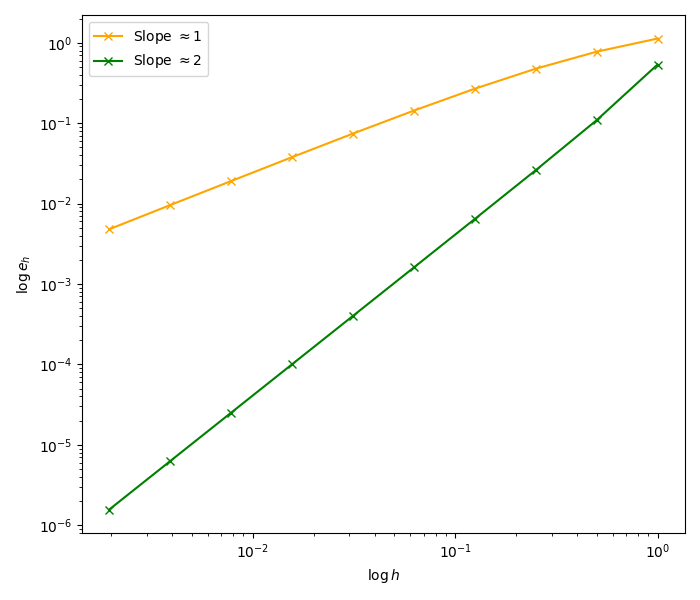
\includegraphics[width=0.9\textwidth]{./img/errors.png}
        \end{center}
    \end{frame}




    \section{Existence and uniqueness of solutions}
    

    \begin{frame}{Picard's theorem}
        Let $f\colon \R^2 \to \R^2$ such that the following properties hold. 
        \begin{enumerate}
            \item $f$ is continuous on $D = [x_0, x_N] \times [y_0 - C, y_0 + C]$.
            \item $|f(x, y_0)| \leq K$ for $x \in [x_0, x_N]$.
            \item $f$ is Lipschitz in the second variable, i.e.\ there exists $L > 0$
            such that for all $x \in [x_0, x_N]$, $u, v \in [y_0 - C, y_0 + C]$,
            we have \[
                |f(x, u) - f(x, v)| \leq L|u - v|.
            \]
            \item \[
                C \geq \frac{K}{L}\left(e^{L(x_N - x_0)} - 1\right).
            \]
        \end{enumerate}
    \end{frame}
    
    \begin{frame}{Picard's theorem}
        Then, there exists a unique function $y \in C^1[x_0, x_N]$ solving the IVP
        \begin{enumerate}
            \item $y(x_0) = y_0$.
            \item $y'(x) = f(x, y)$, on $[x_0, x_N]$
            \item $|y(x) - y_0| \leq C$ on $[x_0, x_N]$
        \end{enumerate}
    \end{frame}

    
    \section{Convergence of iterative methods}

    \begin{frame}{General one-step iterative methods}
        Consider the scheme \[
            y_{i + 1} = y_i + h\cdot \Phi(x_i, y_i; h).
        \] Here, $\Phi$ is continuous in all its variables.

        For example, in Euler's method, \[
            \Phi(x, y; h) = f(x, y).
        \] In the trapezoidal method, \[
            \Phi(x, y; h) = \frac{1}{2}\Big[f(x, y) + f(x + h, y + h\cdot \Phi(x, y;
            h))\Big].
        \] 
    \end{frame}

    \begin{frame}{Global and truncation errors}
        Define the global errors \[
            e_i = y(x_i) - y_i.
        \]

        Define the truncation errors \[
            T_i = \frac{y(x_{i + 1}) - y(x_i)}{h} - \Phi(x_i, y(x_i); h).
        \] 
    \end{frame}

    \begin{frame}{Global and truncation errors}
        Let $\Phi$ be Lipschitz in its second variable, i.e.\ there exists $L_\Phi >
        0$ such that for all $0 \leq h \leq h_0$, \[
            |\Phi(x, u; h) - \Phi(x, v; h)| \leq L_\Phi|u - v|.
        \] Then, assuming that all $|y_i - y_0| \leq C$, \[
            |e_n| \leq \frac{T}{L_\Phi}\left(e^{L_\Phi(x_n - x_0)} - 1\right),
        \] where $T = \max_{0 \leq i < n}|T_i|$.
    \end{frame}

    \begin{frame}{Global and truncation errors}
        The truncation formula can be rearranged as \[
            y(x_{i + 1}) = y(x_i) + h\cdot \Phi(x_i, y(x_i); h) + hT_i.
        \] Subtracting the iteration scheme, we have \[
            e_{i + 1} = e_i + h\cdot \Big[\Phi(x_i, y(x_i); h) - \Phi(x_i, y_i;
            h)\Big] + hT_i.
        \] Use the Lipschitz condition to estimate the bracketed term. \begin{align*}
            |e_{i + 1}| &\leq |e_i| + hL_\Phi|e_i| + h|T_i| \\
            &\leq (1 + hL_\Phi)|e_i| + hT.
        \end{align*}
    \end{frame}

    \begin{frame}{Global and truncation errors}
        Denote $r = 1 + hL_\Phi$.
        \begin{align*}
            |e_0| &= 0, \\
            |e_1| &\leq hT \\
            |e_2| &\leq rhT + hT = (r + 1)hT \\
            |e_3| &\leq r(rhT + hT) + hT = (r^2 + r + 1)hT \\
            \vdots &\qquad \vdots \\
            |e_n| &\leq (r^{n - 1} + r^{n - 1} + \dots + r + 1)hT = hT\cdot \frac{r^n -
            1}{r - 1}.
        \end{align*}
    \end{frame}

    \begin{frame}{Global and truncation errors}
        Use $r = 1 + hL_\Phi \leq e^{hL_\Phi}$, $x_n = x_0 + nh$.
        \[
            |e_n| \leq hT\cdot \frac{e^{nhL_\Phi} - 1}{hL_\Phi} = 
            \frac{T}{L_\Phi}\left(e^{L_\Phi(x_n - x_0)} - 1\right).
        \] 
    \end{frame}

    \begin{frame}{Consistency}
        We demand that the truncation errors vanish as $h \to 0$. In other words, our
        numerical method is said to be consistent with the given ODE if for any
        $\epsilon > 0$, there exists $h_\epsilon > 0$ such that for all $0 \leq h
        \leq h_\epsilon$, we have $|T_i| \leq \epsilon$ for any choice of $0 \leq i <
        N$, any solution curve $y(x)$.

        \[
            T_i = \frac{y(x_{i + 1}) - y(x_i)}{h} - \Phi(x_i, y(x_i); h).
        \] Let $h \to 0$, $N \to \infty$, such that $x_i \to x$. Using the continuity
        of $y, y', \Phi$, we have \[
            0 = y'(x) - \Phi(x, y(x); 0), \qquad \Phi(x, y; 0) = f(x, y).
        \] 
    \end{frame}


    \begin{frame}{Convergence}
        Let our IVP satisfy the conditions of Picard's theorem, let the one-step
        method generate approximations in the region $D$ for all $h \leq h_0$. Recall
        that $\Phi$ is continuous in all its variables, and Lipschitz in the second
        variable. Also suppose that the consistency condition is satisfied. Then, the
        successive approximation sequences $(y_i)$, generated using finer and finer
        meshes (decreasing $h$) converge to the solution of the IVP.

        As $h \to 0$, pick points $x_n \to x \in [x_0, x_N]$ as $n \to \infty$. Then,
        the corresponding $y_n \to y(x)$.
    \end{frame}

    \begin{frame}{Convergence}
        Choose $h \leq h_0$, such that there are $N$ mesh points. Then, \[
            |y(x_n) - y_n| \leq \frac{T}{L_\Phi}\left(e^{L_\Phi(x_N - x_0)} - 1\right).
        \] Use consistency to write \begin{align*}
            T_n &= \frac{y(x_{n + 1}) - y(x_n)}{h} - \Phi(x_n, y(x_n); h) \\
            &= \frac{y(x_{n + 1}) - y(x_n)}{h} - f(x_n, y(x_n)) + \\
            & \qquad\qquad \Phi(x_n, y(x_n); 0) - \Phi(x_n, y(x_n); h) \\
            &= \Big[\frac{y(x_{n + 1}) - y(x_n)}{h} - y'(x_n)\Big] + \\
           & \qquad\qquad  \Big[\Phi(x_n, y(x_n); 0) - \Phi(x_n, y(x_n); h)\Big].
        \end{align*}
    \end{frame}


    \begin{frame}{Convergence}
        Use the Mean Value theorem to choose $\xi_n \in [x_n, x_{n + 1}]$ such that
        $y(x_{n + 1}) - y(x_n) = hy'(\xi_n)$.

        Note that a continuous function on a compact set is also uniformly
        continuous. Thus, we can choose $h_1$ such that for all $h \leq h_1$, \[
            |y'(\xi_n) - y'(x_n)| \leq \frac{1}{2}\epsilon,
        \] and choose $h_2$ such that for all $h \leq h_2$, \[
            |\Phi(x_n, y(x_n); 0) - \Phi(x_n, y(x_n); h)| \leq \frac{1}{2}\epsilon.
        \] Putting $h_\epsilon = \min(h_1, h_2)$, we see that for all $h \leq
        h_\epsilon$, $|T_n| \leq \epsilon$.
    \end{frame}

    \begin{frame}{Convergence}
        Thus, \begin{align*}
            |y(x) - y_n| &\leq |y(x) - y(x_n)| + |y(x_n) - y_n| \\
            &\leq |y(x) - y(x_n)| + \frac{\epsilon}{L_\Phi}\left(e^{L_\Phi(x_N -
            x_0)} - 1\right).
        \end{align*}

        As $n \to \infty$, $x_n \to x$, the continuity of $y$ gives $y(x_n) \to
        y(x)$, making the first term vanish. By making $\epsilon$ arbitrarily small,
        the second term also vanishes. This gives $y_n \to y(x)$, as desired.
    \end{frame}

    \begin{frame}{Application to Euler's method}
        We have \[
            \Phi(x, y; h) = f(x, y).
        \] thus \[
            T_i = \frac{y(x_{i + 1}) - y(x_i)}{h} - y'(x_i).
        \] Assume $y$ is twice continuously differentiable; use Taylor's theorem to
        conclude that \[
            y(x_{i + 1}) = y(x_i) + hy'(x_i) + \frac{1}{2}h^2y''(\xi_i)
        \] for $\xi \in [x_{i}, x_{i + 1}]$, hence \[
            T_i = \frac{1}{2}hy''(\xi_i), \qquad T \leq \frac{1}{2}h\sup|y''(\xi)|.
        \] Thus, the global error obeys \[
            |e_n| \propto T = \mathcal{O}(h).
        \] 
    \end{frame}

    \begin{frame}{Application to the Trapezoidal method}
        We have \[
            \Phi(x, y; h) = \frac{1}{2}\Big[f(x, y) + f(x + h, y + h\cdot \Phi(x, y;
            h))\Big].
        \] To see that $\Phi$ satisfies the Lipschitz condition, we compute 
        \begin{align*}
            |\Phi(x, u; h) &- \Phi(x, v; h)| \\
            \leq& \frac{1}{2}|f(x, u) - f(x, v)| + \\
            &\qquad \frac{1}{2}|f(x, u + h\Phi(x, u; h)) - f(x, v + h\Phi(x, v; h))| \\
            \leq& \frac{1}{2}L|u - v| + \frac{1}{2}L|u - v| +
            \frac{1}{2}Lh|\Phi(x, u; h) - \Phi(x, v; h)|.
        \end{align*}
    \end{frame}

    \begin{frame}{Application to the Trapezoidal method}
        Rearranging, we see that \[
           |\Phi(x, u; h) - \Phi(x, v; h)| \leq \frac{L}{1 - Lh / 2}|u - v|.
        \] For sufficiently small $h$, we have $Lh / 2 < 1$ so choose \[
            L_\Phi \leq \frac{L}{1 - Lh / 2}.
        \] 
    \end{frame}
    
    \begin{frame}{Application to the Trapezoidal method}
        Now, compute the truncation error
        \begin{align*}
            T_i &= \frac{y(x_{i + 1}) - y(x_i)}{h} - \frac{1}{2}\Big[f(x_i, y(x_i))
            + \\
            &\qquad\qquad f(x_i + h, y(x_i) + h\Phi(x_i, y(x_i); h))\Big] \\
            &= \frac{y(x_{i + 1}) - y(x_i)}{h} - \frac{1}{2}\Big[f(x_i, y(x_i)) +
            f(x_{i + 1}, y(x_{i + 1}))\Big] +  \\
            &\qquad \frac{1}{2}\Big[f(x_{i + 1}, y(x_{i + 1})) - f(x_{i + 1}, y(x_i) +
            h\Phi(x_i, y(x_i); h))\Big]
        \end{align*}
    \end{frame}
    
    \begin{frame}{Application to the Trapezoidal method}
        Note that if $y$ is thrice continuously differentiable,
        \begin{align*}
            &\;\frac{y(x_{i + 1}) - y(x_i)}{h} - \frac{1}{2}\Big[f(x_i, y(x_i)) + f(x_{i
            + 1}, y(x_{i + 1}))\Big] \\
            =&\; \frac{y(x_{i + 1}) - y(x_i)}{h} - \frac{1}{2}\Big[y'(x_i) + y'(x_{i +
            1})\Big] \\
            =&\; y'(x_i) + \frac{1}{2}hy''(x_i) + \frac{1}{6}h^2y'''(\xi_i) - \\
            &\qquad \frac{1}{2}\Big[y'(x_i) + y'(x_i) + hy''(x_i) +
            \frac{1}{2}h^2y'''(\zeta_i)\Big] \\
            =&\; \frac{1}{12}h^2\Big[2y'''(\xi_i) - 3y'''(\zeta_i)\Big].
        \end{align*}
    \end{frame}
    
    \begin{frame}{Application to the Trapezoidal method}
        For the final term, use the Lipschitz condition to estimate
        \begin{align*}
            &\frac{1}{2}|f(x_{i + 1}, y(x_{i + 1})) - f(x_{i + 1}, y(x_i) + h\Phi(x_i, y(x_i);
            h))| \\
            \leq\; &\frac{1}{2}L|y(x_{i + 1}) - y(x_i) - h\Phi(x_i, y(x_i); h)| \\
            =&\; \frac{1}{2}Lh|T_i|.
        \end{align*}
    \end{frame}

    \begin{frame}{Application to the Trapezoidal method}
        Further imposing $Lh / 2 < 1 / 2$, we can put these together to get
        \begin{align*}
            |T_i| &\leq \frac{1}{12}h^2|2y'''(\xi_i) - 3y'''(\zeta_i)| +
            \frac{1}{2}Lh|T_i|, \\
            T & \leq \frac{5}{6}h^2 \sup|y'''(\zeta)|.
        \end{align*}
        
        Thus, the global error obeys \[
            |e_n| \propto T = \mathcal{O}(h^2).
        \] 
    \end{frame}
    
\end{document}
% vim: set tabstop=4 shiftwidth=4 softtabstop=4:
